%%%%%%%%%%%%%%%%%%%%%%%%%%%%%%%%%%%%%%%%%%%%%%%%%%%%%%%%%%%%%%%%%%%%%%%%%%%%%%%%
\chapter{Анализ методик и систем диагностирования систем хранения данных}
%%%%%%%%%%%%%%%%%%%%%%%%%%%%%%%%%%%%%%%%%%%%%%%%%%%%%%%%%%%%%%%%%%%%%%%%%%%%%%%%
\section{Системы хранения данных}
Объектом исследования данной работы являются системы хранения данных(СХД). Рассмотрим подробнее их разновиднсти и устройство. 
Традиционно выделяют четыре технологии организации систем хранения данных: 
\begin{itemize*}
	\item{Direct Attached Storage(DAS) - непосредственное подключение носителя,}
	\item{Network Attached Storage(NAS) - сетевая подсистема хранения даннных,}
	\item{Storage Area Network(SAN) - сеть хранения данных,}
	\item{Unified - универсальные системы.}
\end{itemize*}

\begin{figure}[!h]
	\centering
	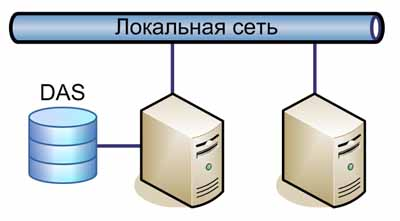
\includegraphics[width=2.0in]{DAS}
	\caption{Архитектура DAS систем}
	\label{fig:DAS}
\end{figure}

DAS- архитектурное решение, предполагающее непосредственное подключение устройства хранения к серверу, который управляет работой системы хранения данных. Основными преимуществами таких систем являются низкая стоимость и простота самой системы, а также ее обслуживания. Основным недостатком системы является неоптимальное использование ресурсов в случае увеличения системы, так как к каждой такой системе требуется выделенный сервер. Архитектура таких систем представлена на рисунке~\ref{fig:DAS}. Представителем таких систем является семейство DELL PowerVault серии MD.

NAS - это решение, предоставляющее доступ к данным через локальную сеть. В настоящее время практически все NAS устройства ориентированы на использование в сетях Ethernet (Fast Ethernet, Gigabit Ethernet) на основе протоколов TCP/IP. Сетевой доступ к данным производится с помощью специальных протоколов доступа к файлам: CIFS, NFS и DAFS. Отличительной особенностью системы является то, что операции в системе выполняются с файлами. Внутри подобных серверов стоят специализированные ОС(MS Windows Storage Server и др.). Архитектура таких систем представлена на рисунке~\ref{fig:NAS}.

\begin{figure}[!h]
	\centering
	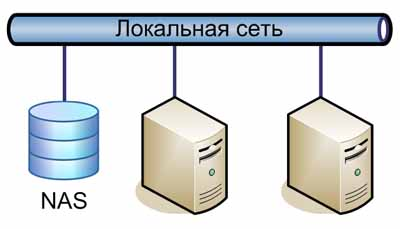
\includegraphics[width=2.0in]{NAS}
	\caption{Архитектура NAS систем}
	\label{fig:NAS}
\end{figure}
  
SAN - это сеть, объединяющая устройства хранения данных с серверами приложений. В отличие от NAS, SAN не оперирует с файлами: файловые операции выполняются на подключенных к SAN серверах, а сама сеть оперирует блоками данных. Оконечные элементы SAN - это серверы приложений и системы хранения данных между которыми, как и в обычной сети, находятся коммутаторы, адаптеры и пр.

\begin{figure}[!h]
	\centering
	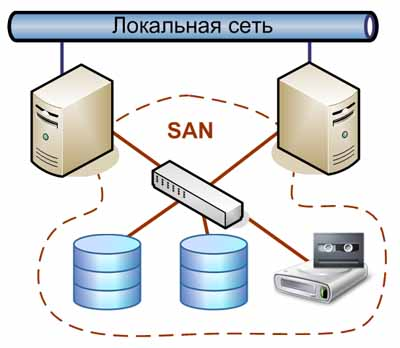
\includegraphics[width=2.0in]{SAN}
	\caption{Архитектура SAN систем}
	\label{fig:SAN}
\end{figure}

SAN системы обычно строятся на основании одного из протоколов: Fibre Channel или ISCSI. Архитектура SAN систем представлена на рисунке~\ref{fig:SAN}.

Unified системы совмещают в себе технолоии NAS и SAN систем, и позволяют использовать как блочный так и файловый тип доступа к ресурсам. 

В системе любой из вышерассмотренных архитектур основным элементом является JBOD - дисковый массив, так как именно на дисках хранится информация. Для повышения надежности данного узла и всей системы в целом производители систем хранения данных разрабатывают системы диагностики СХД. Ключевой составляющей диагностики любой системы является мониторинг значений ее параметров. 

Средства, с помощью которых можно осуществлять мониторинг параметров систем хранения данных можно сгруппировать следующим образом:
\begin{itemize*}
	\item{Программные решения:}
	\begin{itemize*}
		\item{Специальные системы мониторинга}
		\item{Системы мониторинга общего назначения}
	\end{itemize*}
	\item{Аппаратные решения}
\end{itemize*}

Рассмотрим подробнее наиболее характерных представителей каждой группы.
 
%%%%%%%%%%%%%%%%%%%%%%%%%%%%%%%%%%%%%%%%%%%%%%%%%%%%%%%%%%%%%%%%%%%%%%%
\section{Специальные системы мониторинга}
Данные системы разработаны самими  производителями систем хранения данных и чаще всего поставляются в комплекте с СХД.

Первым представителем сипециальных систем мониторинга является система мониторинга параметров СХД IBM Spectrum от фирмы IBM. Позволяет уведомлять об изменении состояния компонента и отслеживать состояние компонентов визуально. Пользовательский интерфейс системы представлен на рисунке~\ref{fig:Spectrum}.
\begin{figure}[!h]
	\centering
	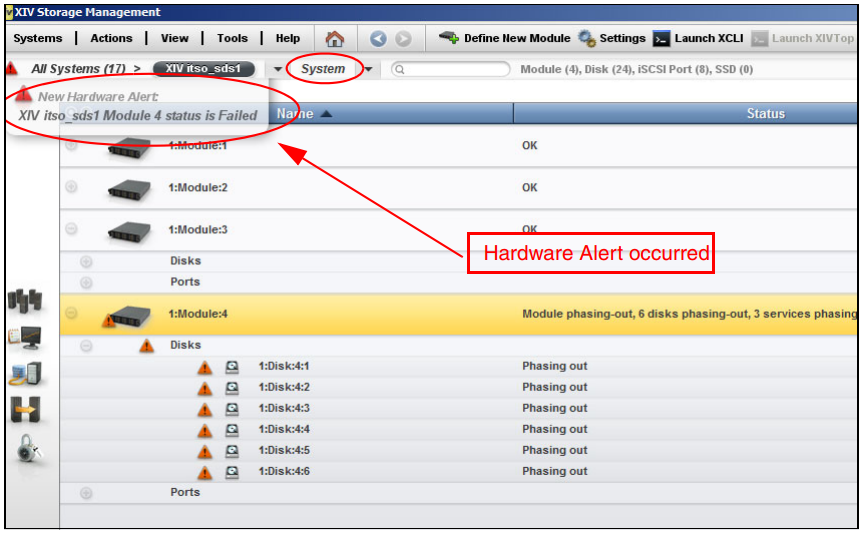
\includegraphics[width=\textwidth]{Spectrum}
	\caption{Пользовательский интрефейс IBM Spectrum}
	\label{fig:Spectrum}
\end{figure}

В системе предполагается градация по пяти уровням критичности произошедшего события~\cite{Spectrum}. Уровни градации представлены на рисунке~\ref{fig:Spectrum2}.
\begin{figure}[!h]
	\centering
	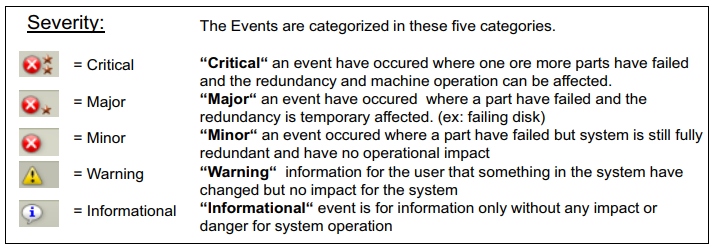
\includegraphics[width=\textwidth]{Spectrum2}
	\caption{Градация сообщений системы Spectrum}
	\label{fig:Spectrum2}
\end{figure}
Среди достоинств системы можно отметить широкую классификацию событий и понятный пользователю интерфейс. Основным недостатком системы является большая ориентированность на скоростные, стоимостные и нагрузочные показатели, нежели на характеристику компонентов и системы в целом. 

Еще одним представителем данной группы является система мониторинга и информирования EMC VNX от EMC~\cite{EMC}, предоставляемая совместно с оборудованием. Позволяет в графическом виде наблюдать структуру системы, нагрузку на компоненты, активность сервисов системы. 
\begin{figure}[!h]
	\centering
	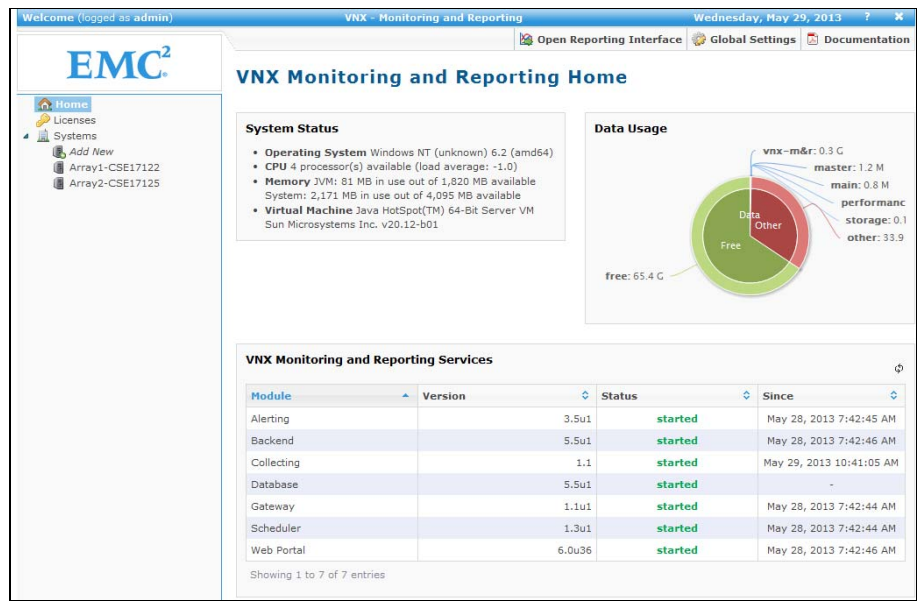
\includegraphics[width=\textwidth]{EMC}
	\caption{Пользовательский интрефейс EMC VNX}
	\label{fig:EMC}
\end{figure}
Аналогично системе Spectrum, используются информирующие сообщения пяти уровней критичности, но имеется возможность уведомления о событиях на электронную почту. Кроме того, в системе присутствует большое количество сетевых и системных настроек, позволяющих создавать кластеры, размечать диски, настраивать доступы и сети. Таким образом, система является в большей степени комплексной,а задача мониторинга состояния компонентов не является основопологающей. 

Еще одна специальная система мониторинга разработана компанией FUJITSU - ServerView System Monitor~\cite{Fujitsu}. Система является визуализатором дерева подкомпонентов системы с состоянием каждого. Пользовательский интерфейс представлен на рисунке~\ref{fig:Fujitsu}.  
\begin{figure}[!h]
	\centering
	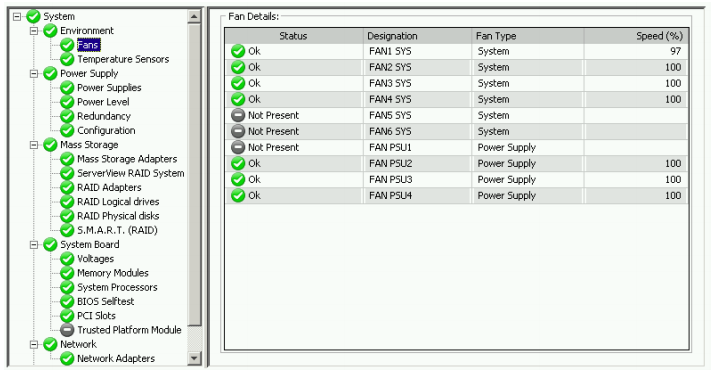
\includegraphics[width=\textwidth]{Fujitsu}
	\caption{Пользовательский интрефейс FUJITSU Server View}
	\label{fig:Fujitsu}
\end{figure}
Кроме десктопного исполнения FUJITSU разработала мобильное приложение, с аналогичной функциональностью (см. рисунок ~\ref{fig:Fujitsu2}).
\begin{figure}[!h]
	\centering
	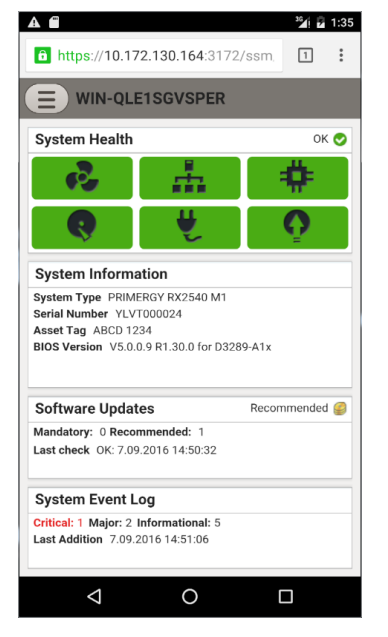
\includegraphics[width=2.0in]{Fujitsu2}
	\caption{Мобильное приложение от Fujitsu}
	\label{fig:Fujitsu2}
\end{figure}

Преимуществом данной системы по сравнению с ранее рассмотренными является большее уделение внимания состоянию системы в целом и компонентов в частности. Дерево компонентов системы позволяет быстро оценить состояние каждого,а при необходимости раскрыть и узнать большее количество информации, вплоть до причины возникновения ошибки. Кроме того, разработанное мобильное приложение позволяет администратору быть в курсе событий даже если он не находится непосредственно на рабочем месте. 
%%%%%%%%%%%%%%%%%%%%%%%%%%%%%%%%%%%%%%%%%%%%%%%%%%%%%%%%%%%%%%%%%%%%%%%
\section{Системы мониторинга общего назначения}
Представителями второй группы являются Elastic, Zabbix и Anomaly. Данные системы разрабатываются отдельно от систем хранения данных и предназначены для решения более общих задач, таких как сбор данных с большого количества источников, обработка данных, визуализация и поиск аномалий. 

Первая из рассматриваемых - система Elastic представляет из себя свободно распространяемый стек программ, предназначенный для сбора, хранения, обработки и отображения данных из разных источников. 
Состав программных продуктов Elastic представлен ниже: 
\begin{itemize*}
	\item{Elasticsearch – поисковая система с открытым исходным кодом, использует REST интерфейс и оперирует данными в формате JSON}
	\item{Kibana – инструмент позволяющий визуализировать данные в виде графиков, статистики и пр.}
	\item{Logstash - конвейер обработки данных на стороне сервера, который получает данные из нескольких источников одновременно, преобразует их, а затем отправляет в хранилище, например Elasticsearch}
	\item{Beats - платформа для легковесной отправки данных. Существует возможность отправлять данные с тысяч машин и систем в Logstash, используется для сбора данных}
	\item{ECE - Elastic Cloud Enterprise – предоставляет доступ для управления и контроля Elasticsearch и Kibana в любой инфраструктуре, управляя всем с одной консоли}
	\item{Machine learning – часть программного пакета X-Pack. Основной возможностью продукта является обнаружение аномалий временных рядов с использованием машинного обучения.}
\end{itemize*}

Наиболее интересным с точки зрения мониторинга параметров является последний пакет. Наилучшим применением данной технологии является обнаружение отклонений в значениях некоторых величин от нормального поведения. Чаще всего для этих целей используют правила, пороговые значения и различные простые статические методы. Однако такие способы зачастую неэффективны, так как они основываются на неверных статистических допущениях (Гауссово распределение и др.), а также не учитывают тренды (долгосрочное или периодическое изменение сигнала). Еще одним преимуществом пакета является возможность совместного анализа большого количества метрик, выявляя неявные зависимости. Предоставляется возможность вывода информации о всех аномалиях на один общий график. Анализ данных производится в реальном времени, возможно оповещение об обнаруженных аномалиях. Пакет полностью бесплатен начиная с 7 сентября 2018 года. 


\begin{figure}[htbp]
	\centering
	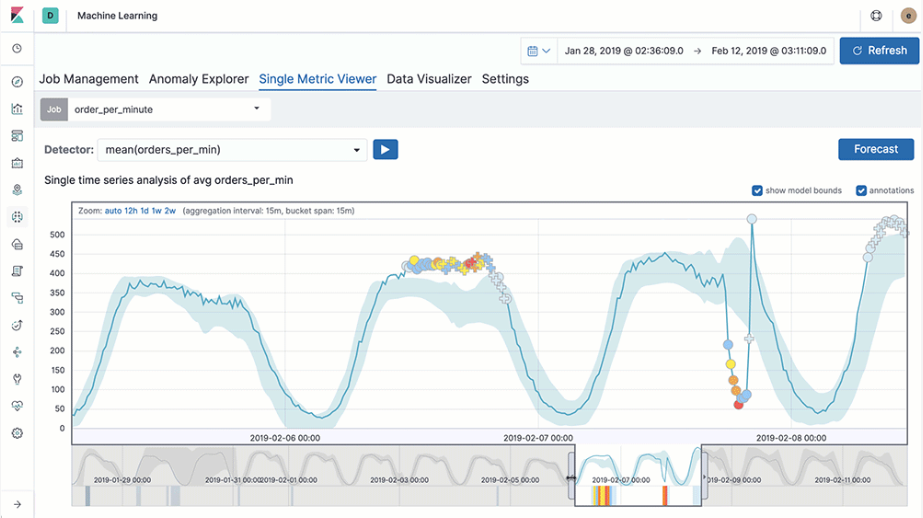
\includegraphics[width=\textwidth]{Elastic}
	\caption{Обнаружение аномалий в Elastic}
	\label{fig:Elastic}
\end{figure}

Еще один представитель второй группы - Zabbix. Это программное обеспечение для мониторинга параметров сети, жизнеспособности и целостности серверов. Zabbix состоит из нескольких компонентов:
\begin{itemize*}
	\item{сервер мониторинга, который выполняет периодическое получение данных, обработку, анализ и запуск скриптов оповещения}
	\item{агенты - демоны, которые запускаются на отслеживаемых объектах и предоставляет данные серверу}
	\item{база данных (MySQL, PostgreSQL, SQLite или Oracle) для хранения накопленной информации}
	\item{веб-интерфейс на PHP, предоставляющий информацию о производительности и состоянии системы}
\end{itemize*}

\begin{figure}[!htbp]
	\centering
	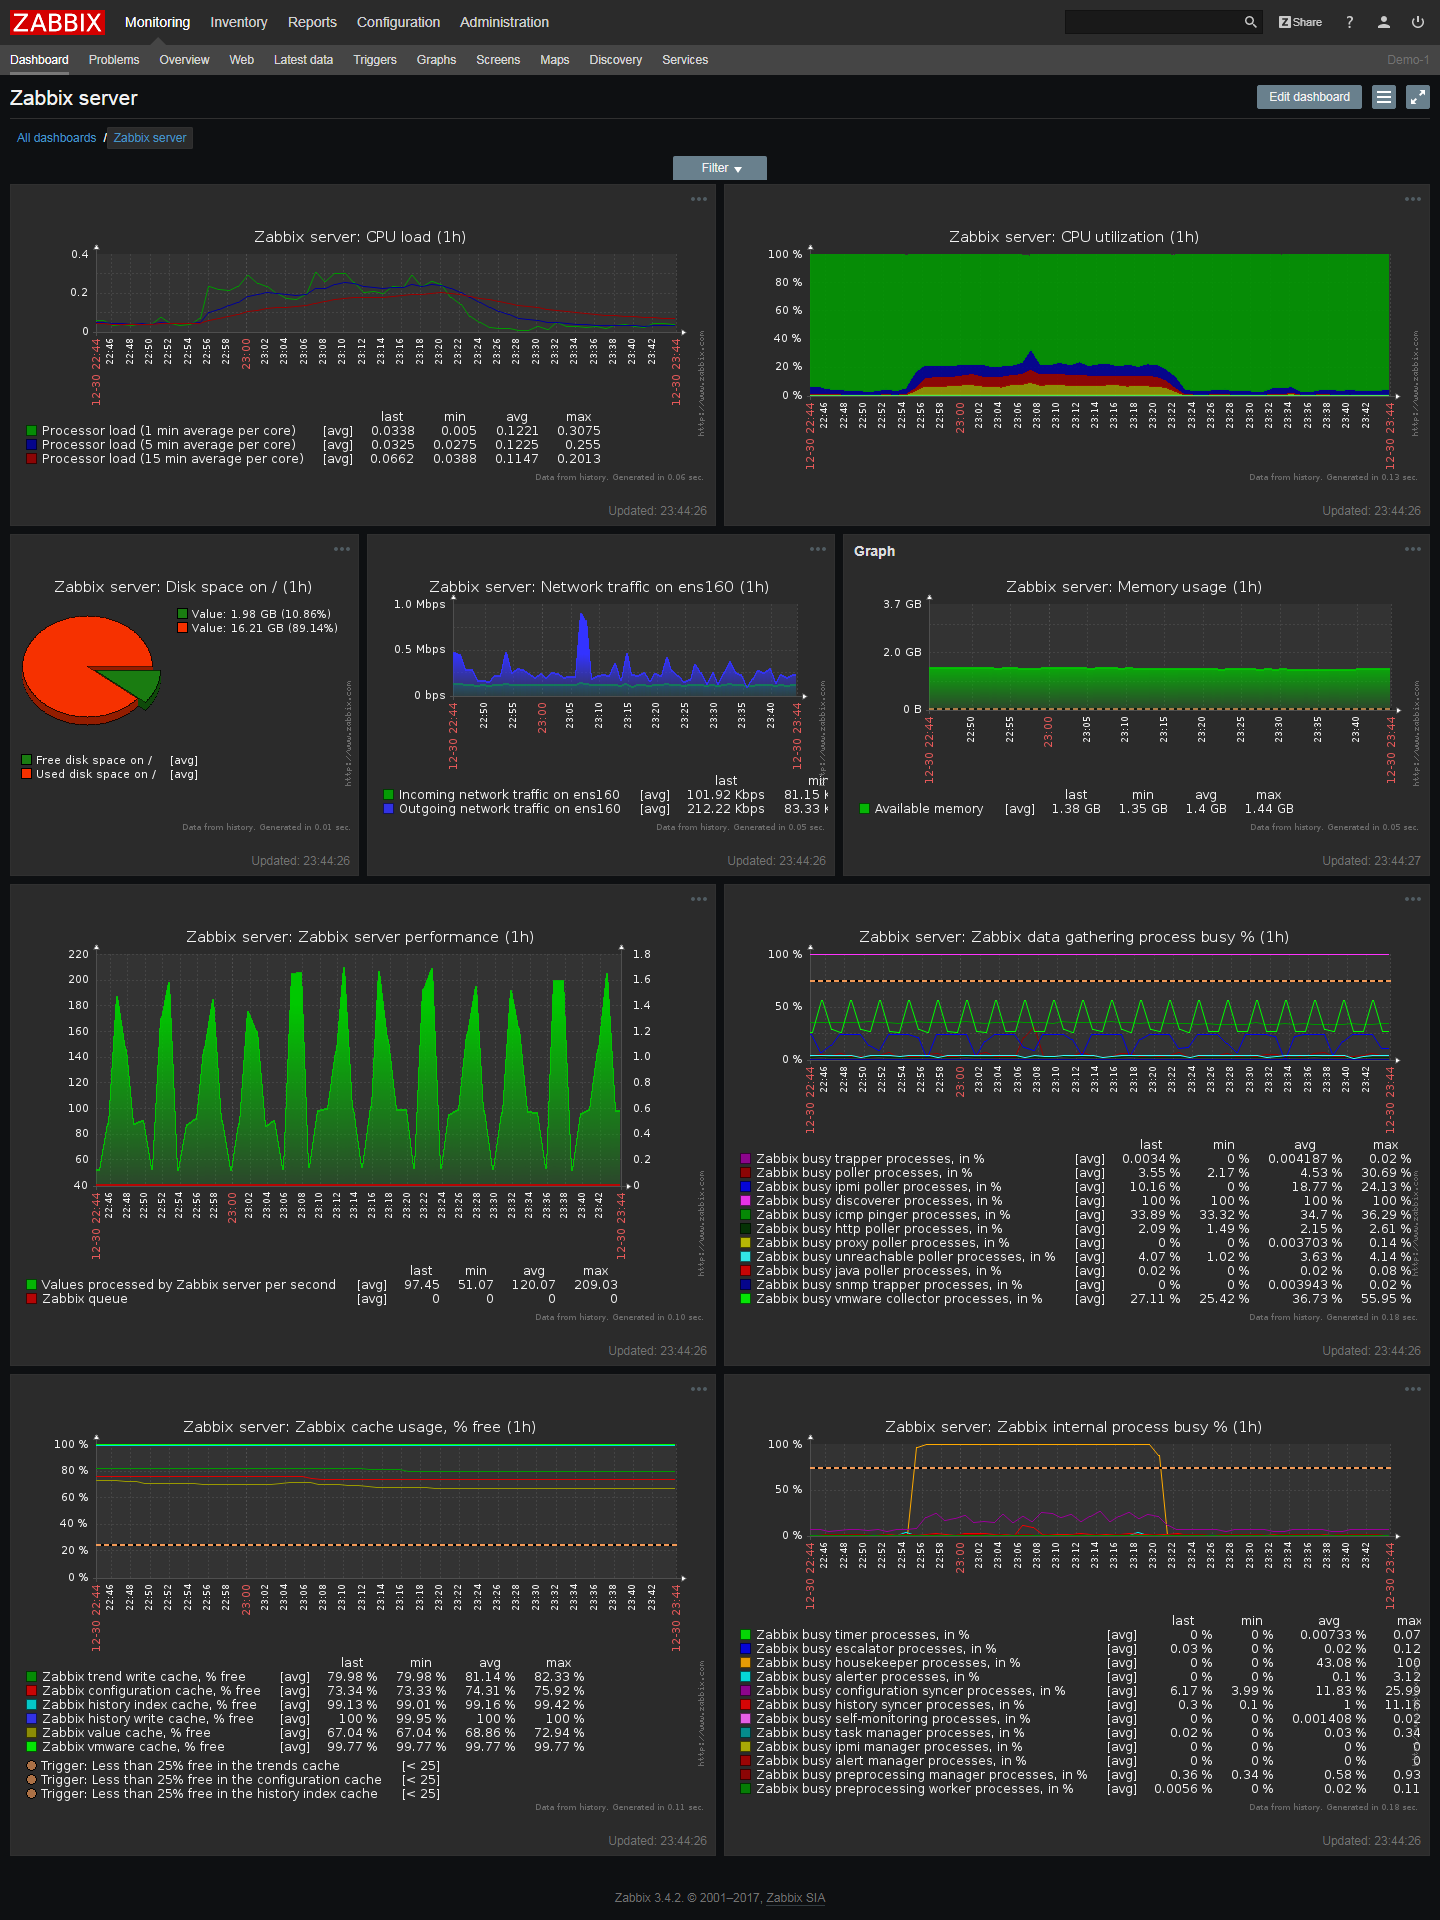
\includegraphics[width=\textwidth]{Zabbix}
	\caption{Отображение парметров в графическом виде в системе Zabbix}
	\label{fig:Zabbix}
\end{figure}

Преимуществом системы является возможность работаты без агента. Для этого используются общие протоколы мониторинга, такие как протокол управления сетью.  Кроме того, мониторинг можно производить с помощью запуска внешних скриптов, встроенных проверок (http запрос, ping и др). Недостатком системы явялется то, что продукт является коммерческим, а значит нет возможности собственной доработки и его продажи совместно с другими собственными продуктами.  

Последний рассматриваемый представитель второй группы - Anomaly. Anomaly представляет из себя сервис по диагностированию аномалий в реальном времени~\cite{Anomaly}. Данные для мониторинга загружаются в облако, где после обработки и процесса обучения становится доступным детектирование отклонений в поведении (см. рисунок ~\ref{fig:Anomaly}). При этом процесс обучения не останавливается и длится постоянно. После первичного обучения алгоритмы формируют простые паттерны определения ошибок, такие как максимумы и минимумы. Со временем происходит детализирование и выявление корреляций, трендов и др. Для обучения используется машинное обучение, нейронные сети, собственные математические модели. 
\begin{figure}[!h]
	\centering
	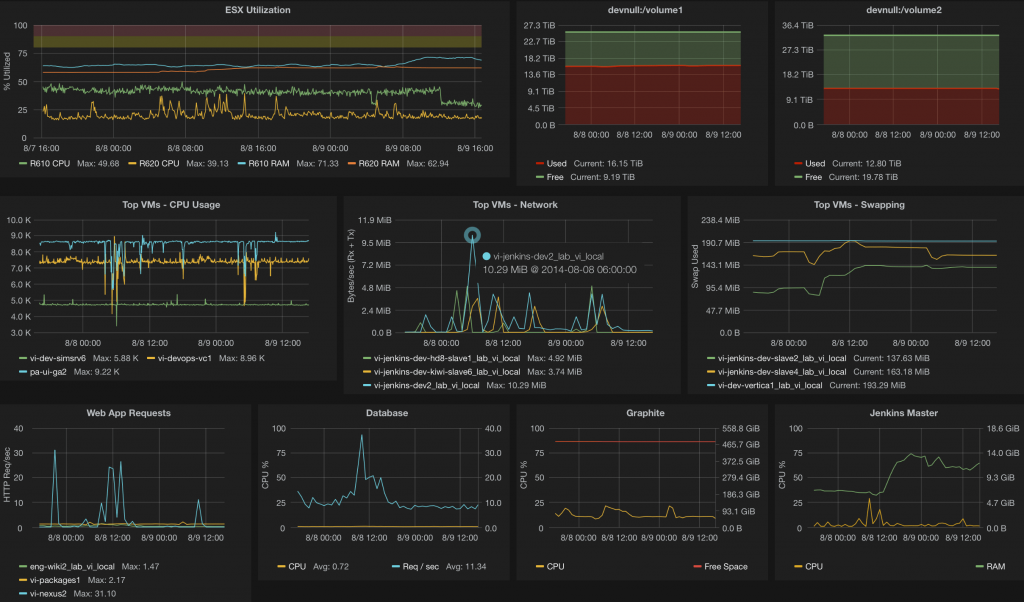
\includegraphics[width=\textwidth]{Anomaly}
	\caption{Пользовательский интерфейс Anomaly}
	\label{fig:Anomaly}
\end{figure}

При обнаружении аномалии пользователю отправляется сообщение (смс, почта) или выполняется собственно-назначенное действие. Система является коммерческим продуктом. Недостатком системы является удаленное расположение сервера обработки данных. В случае закрытых ЦОД или иных ограниченных доступом систем данное решение не применимо. Кроме того, в случае использования такой системы появляется необходимость транзита большого количества данных по сети, что увеличивает загрузку на сеть. Однако, использование сторонних серверов для обработки данных позволяет экономить собственные вычислительные ресурсы. 

\section{Аппаратные решения}
Рассмотрим аппаратные решения, применяемые в мониторинге параметров систем хранения данных. 

\begin{figure}[!h]
	\centering
	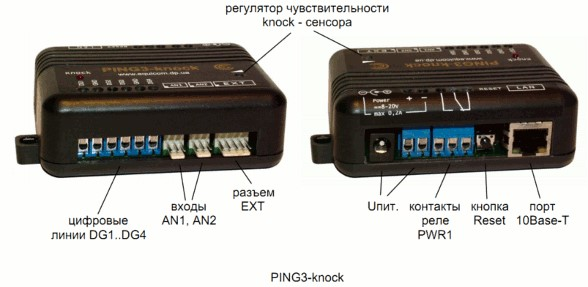
\includegraphics[width=\textwidth]{monitoring_temperature}
	\caption{Аналог разрабатываемой системы от EQUICOM}
	\label{fig:monitoring_temperature}
\end{figure}

Система мониторинга датчиков в серверной фирмы EQUICOM.

Предоставляет возможность подключения датчиков температуры(до 2шт), напряжения, дыма, удара и протечки воды. Среди преимуществ системы можно отметить низкую стоимость(менее 6 тысяч рублей за устройство и 4 датчика),наличие web интерфейса управления устройством и протокола обмена данными. Недостатками системы являются негабаритный форм-фактор корпуса(не 1U),отсутствие графической визуализации показаний, отсутствие хранения истории  данных, высокая стоимость дополнительных датчиков(1-2 тысячи рублей), отсутствие датчика влажности, вибрации и давления~\cite{analog1}. Внешний вид системы приведен на рисунке~\ref{fig:monitoring_temperature}.

\begin{figure}[!h]
	\centering
	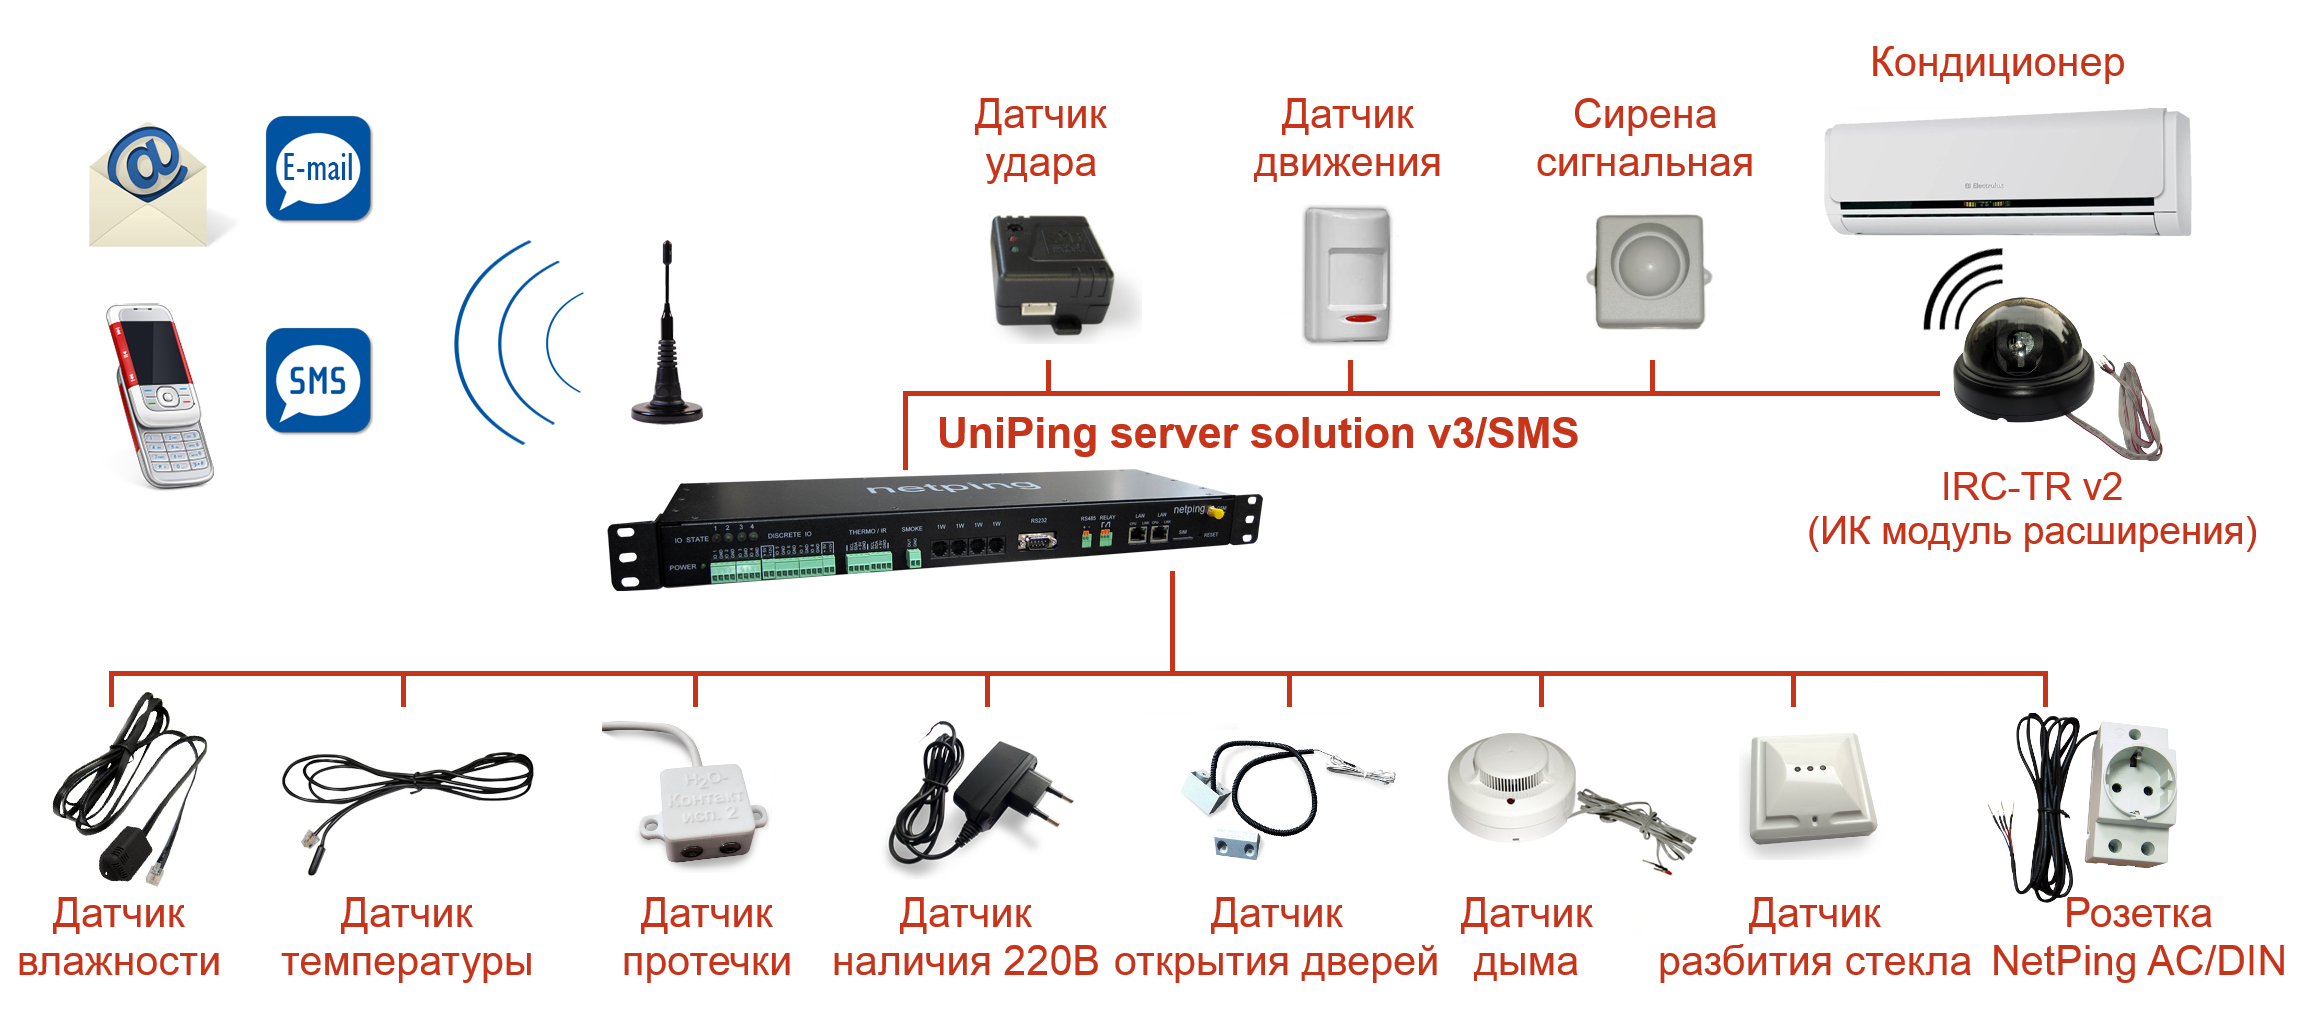
\includegraphics[width=\textwidth]{analog2}
	\caption{Аналог разрабатываемой системы от  UniPing}
	\label{fig:analog2}
\end{figure}

Система UniPing server solution v3/SMS~\cite{analog2} является комплексным решением для мониторинга серверной с большим колчичеством подключаемых датчиков и устройств. Среди преимуществ системы можно выделить: мониторинг климатических параметров помещения, наличия движения, контроль доступа к помещению, возможность управления кондиционером, отправки уведомлений и форм-фактор основного изделия, позволяющий встроить  соновной модуль в стойку(1U). К недостаткам системы относятся высокая стоимость(более 32 тысяч рублей), отсутствие хранения истории данных, отсутствие датчика давления, вибрации, отсутствие графической визуализации показаний. Внешний вид системы приведен на рисунке~\ref{fig:analog2}.  

\section{Сравнительный анализ систем мониторинга и подходов к диагностике}

Резюмируя вышесказанное можно заключить, что существует большое количество различных систем мониторинга параметров, однако они обладают рядом недостатков:
\begin{itemize*}
	\item{Системы, поставляющиеся с оборудованием от производителя, работают только с их оборудованием, и, зачастую, не отображают данные в удобном виде}
	\item{Системы общего назначения максимально унифицированы под сбор и визуализацию всевозможных данных, поэтому такие системы не отображают иерархически компоненты системы, что усложняет определение последствий возникновения аномалий.  Кроме того, зачастую такие системы расположены на удалённых серверах, что делает невозможным их применение в закрытых(изолированных) решениях.}
\end{itemize*}

Рассмотренные аппаратные решения обладают рядом недостатков, не позволяющих их использовать в качестве полноценной подсистемы сбора и визуализации климатических параметров в комплексе мониторинга и диангостики систем хранения данных (отсутствие необходимых датчиков давления и вибрации, отсутствие графической визуализации показаний, отсутствие хранения истории показаний, высокая стоимость для некоторых систем).

В рассмотренных выше системах применялись различные методики обнаружения сбоев в системе, а именно:
\begin{itemize*}
	\item{Событийные системы, с заранее заданными производителем событиями. Уведомления происходят в моменты наступления событий.}
	\item{Обнаружение сбоев на основе пользовательского списка правил(указание граничных значений параметров и их комбинаций)}
	\item{Обучение интеллектуальных алгоритмов определения аномалий с последующим постоянным дообучением в процессе работы}
	\item{Сопоставление топологии системы в текущей конфигурации с получаемыми данными мониторинга с целью определением перечня неисправных компонентов.}
\end{itemize*}
Наиболее перспективными подходами кажутся последние два, применяемые совместно, так как они позволяют автоматизировать процесс поиска сбоев, а также наиболее точно указывать на сбойный компонент. 

\section{Постановка задачи}

Таким образом, актуальной является задача разработки собственной системы мониторинга и диагностики СХД. В рамках одного из проектов научной лаборатории НИЛ АСПОД в СПбПУ разрабатывается такая система. Структура разрабатываемой системы приведена на рисунке ~\ref{fig:diagSystem}.
\begin{figure}[!h]
	\centering
	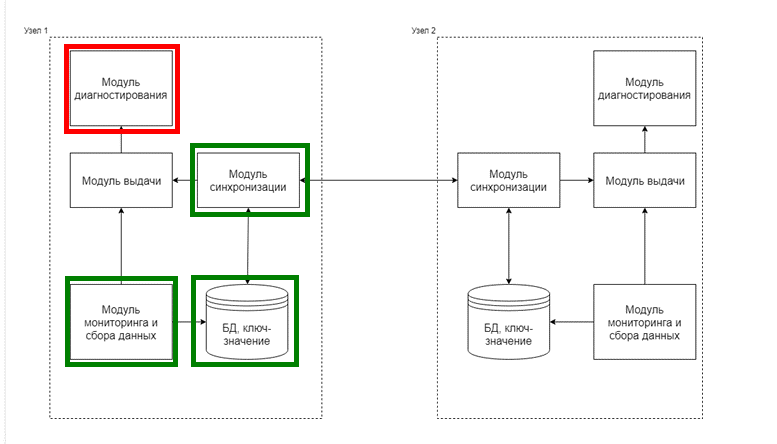
\includegraphics[width=\textwidth]{diagSystem}
	\caption{Структура разрабатываемой в лаборатории системы мониторинга и диагностики}
	\label{fig:diagSystem}
\end{figure}

Зелёным цветом выделены ранее реализованные модули.
В данной работе рассматривается ряд прикладных задач в рамках работы над модулем диагностирования. В частности, формулируется задача разработки методики диагностики состояний системы хранения данных, что предполагает решение ряда задач:
\begin{itemize*}
	\item{Анализ объекта диагностики}
	\item{Определение параметрического пространства для объекта диагностики}
	\item{Описание возможных состояний объекта диагностики}
	\item{Определение значений параметров соответствующих различным состояниям объекта диагностики}
	\item{Формирование диагностической модели}
\end{itemize*}
Кроме того, с целью обеспечения полноты собираемых параметров, формулируется задача разработки и изготовления аппаратно-программного комлекса сбора и отображения климатических параметров СХД. Для достижения поставленной цели необходимо решить ряд задач: 
\begin{itemize*}
	\item{Разработка структуры комплекса}
	\item{Разработка и реализация аппаратной части}
	\item{Проведение исследовательских испытаний}
\end{itemize*}	 

 
%%\begin{table}
% Для таблиц с multirow и multicol необходимо вручную указать сдвиг для caption
%%\captionsetup{skip=5pt}
%%\caption{Example}
%%\centering
%%\begin{tabular}{|r|c|c|c|c|c|c|}
%%\hline
%%            \multirow{2}{*}{}
%%           & \multicolumn{2}{c|}{LLVM IR} 
%%           & \multicolumn{2}{c|}{PS} 
%%           & \multicolumn{2}{c|}{AI} \\ \cline{2-7}
%%           & SAT    & UNSAT   & SAT    & UNSAT   & SAT    & UNSAT   \\ \hline
%%beanstalkd & 356    & 252     & 360    & 161     & 360    & 247     \\ \hline
%%clib       & 599    & 258     & 960    & 234     & 960    & 449     \\ \hline
%%\end{tabular}
%%\label{table:checkResults}
%%\end{table}

%%%%%%%%%%%%%%%%%%%%%%%%%%%%%%%%%%%%%%%%%%%%%%%%%%%%%%%%%%%%%%%%%%%%%%%%%%%%%%%%
%%\section{bar}
%%%%%%%%%%%%%%%%%%%%%%%%%%%%%%%%%%%%%%%%%%%%%%%%%%%%%%%%%%%%%%%%%%%%%%%%%%%%%%%%

%%\blindtext
%%It is of great importance that you use correct references in your dissertation.
%%Resent studies show that it can increase the chances of successful defense
%%by as much as 3,17 percent~\cite{russian, java-book}.

%%\begin{table}[H]
%%	\caption{Название таблицы}
%%	\begin{center}
%%		\begin{tabular}{|l|l|}
%%			\hline
%%			top left & top right\\ \hline
%%			bot left & bot right\\ \hline
%%		\end{tabular}
%%		\label{tabular:tab_examp}
%%	\end{center}
%%\end{table}


